\documentclass[10pt,journal]{IEEEtran}
\usepackage[spanish]{babel}
\usepackage[T1]{fontenc}
\usepackage{amsmath}
\usepackage{amssymb}
\usepackage{float}
\usepackage{graphicx}
\usepackage{booktabs}
\usepackage{placeins}
\usepackage{xcolor}
\usepackage{listings}

\lstdefinestyle{pythonstyle}{
  language=Python,
  basicstyle=\ttfamily\small,
  keywordstyle=\color{blue!60!black}\bfseries,
  stringstyle=\color{red!50!brown},
  commentstyle=\color{gray}\itshape,
  numbers=none,
  breaklines=true,
  showstringspaces=false,
  frame=single,
  framesep=3pt,
  xleftmargin=3pt,
  xrightmargin=3pt,
  columns=flexible,
}
\lstset{style=pythonstyle}
\usepackage[pdfauthor={Jheison Martinez Bolivar},pdftitle={Series Temporales: Actividad Solar y Temperatura Global con ARIMA, LSTM y DQN},colorlinks,linkcolor=blue,citecolor=green,urlcolor=cyan]{hyperref}

\newcommand{\enlacenb}{\url{https://colab.research.google.com/github/JheisonMB/ml/blob/main/series-temporales-prediccion/series_temporales_prediccion.ipynb}}

\begin{document}

  \title{Series Temporales: \textquestiondown{}La Actividad Solar Ayuda a Predecir la Temperatura Global?\\ ARIMA, LSTM y DQN sobre Manchas SILSO y Anomal\'ias Berkeley Earth}

  \author{
    Jheison Martinez Bolivar\\
    \textit{Maestr\'ia en Inteligencia Artificial}\\
    \textit{Universidad de La Salle, Bogot\'a, Colombia}\\
    \texttt{jhmartinez07@unisalle.edu.co}
  }
  \maketitle
  \markboth{Universidad de La Salle --- Aprendizaje de M\'aquina. Septiembre 2026}{}

  \begin{abstract}
    Este trabajo pregunta si la actividad solar aporta se\~nal predictiva a la temperatura global mensual. Sobre el marco com\'un 1880--2025 (1\,751 meses, sin nulos ni duplicados) se compara la anomal\'ia terrestre \texttt{land} de Berkeley Earth contra el conteo de manchas SILSO como variable ex\'ogena, con corte temporal en 2001 (entreno $n=1\,452$, prueba $n=299$). El ARIMA(2,1,1) elegido por AIC obtiene $RMSE=0.4637$ en la prueba; a\~nadir el sol lo empeora ($RMSE=0.5121$, $\beta=-6.07\times10^{-6}$ con $p=0.96$). La LSTM univariada empata al ARIMA ($RMSE=0.4799$) y la multivariada pierde en las tres semillas ($RMSE$ entre 0.50 y 1.05), as\'i que la hip\'otesis solar queda enterrada por las dos v\'ias. La misma tabla incluye la l\'inea base que ning\'un modelo supera: la persistencia marca $RMSE=0.1216$, casi cuatro veces mejor que el ARIMA, de modo que el objeto del trabajo no es predecir la temperatura sino medir lo que cuesta a\~nadir el sol. En bloque aparte, un DQN con acciones discretizadas aprende a estabilizar el p\'endulo de \texttt{Pendulum-v1} (retorno voraz $-200\pm38$ entre tres semillas contra $-1\,170\pm238$ del azar). El cuaderno con la implementaci\'on completa se ejecuta en Colab desde \enlacenb.
  \end{abstract}

  \section{Introducci\'on}

  \IEEEPARstart{E}{l} Sol impone un ciclo de unos once a\~nos sobre su propia actividad, visible en el conteo de manchas \cite{hathaway2015}, y el clima terrestre guarda memoria de largo plazo en sus anomal\'ias de temperatura \cite{silso2025,berkeleyearth2024}. La pregunta de si el primero ayuda a predecir la segunda es anterior al aprendizaje autom\'atico y sigue abierta en su forma predictiva: no si el Sol causa el clima, sino si ver las manchas reduce el error de pron\'ostico de la temperatura.

  Este trabajo la convierte en una comparaci\'on cerrada: la misma serie, el mismo corte temporal, los mismos errores, con y sin la variable solar. Del lado estad\'istico, ARIMA y su extensi\'on con ex\'ogena ARIMAX \cite{box2015}; del lado aprendido, redes LSTM univariadas y multivariadas \cite{hochreiter1997,lim2021}. En bloque independiente, y porque la actividad tambi\'en lo pide, un agente DQN \cite{mnih2015} sobre un entorno de control continuo. La metodolog\'ia de series sigue la referencia can\'onica de pron\'ostico \cite{hyndman2021}.

  \section{Datos y Preprocesamiento}

  \subsection{Selecci\'on de los Conjuntos de Datos}

  Se usan dos fuentes con cobertura mensual solapada desde 1880. Las manchas provienen del conteo mensual total SILSO v2.0 \cite{silso2025}: el observatorio lo distribuye en texto de ancho fijo y son siete columnas \cite{silso2025}, y el archivo que se usa aqu\'i, \texttt{SN\_m\_tot\_V2.0.csv} sin encabezado y con separador \texttt{;}, es la copia tabular de la plataforma de cursos \cite{kaggle_sunspot_dataset}. La temperatura proviene de las anomal\'ias mensuales Berkeley Earth (columnas \texttt{time}, \texttt{station}, \texttt{land}), donde cada valor es la desviaci\'on del mes respecto a su referencia clim\'atica de 1951--1980 \cite{berkeleyearth2024,rohde2020,kaggle_land_temperature_dataset}. Una anomal\'ia no es la temperatura del term\'ometro: $+0.5$ significa medio grado por encima de lo normal para ese mes.

  Como protagonista se fija \texttt{land} (solo tierra): trae menos dispersi\'on que la combinada \texttt{station} ($\sigma=0.41$ contra $0.52$) y es la serie limpia del conjunto; su correlaci\'on mensual contempor\'anea con las manchas es pr\'acticamente cero en ambas ($\approx 0.02$), as\'i que un v\'inculo instant\'aneo queda descartado desde el EDA.

  \subsection{Marco Com\'un y Limpieza}

  El tiempo decimal de Berkeley Earth se convierte a mes calendario por truncamiento, no por redondeo: redondear salta febrero y duplica abril, defecto que se detect\'o por 585 fechas duplicadas y se corrigi\'o antes de seguir. El marco com\'un 1880-01 a 2025-11 queda con $n=1\,751$ meses contiguos, cero nulos y cero duplicados. La Figura~\ref{fig:nivel} muestra las dos series en nivel.

  \begin{figure*}[t]
    \centering
    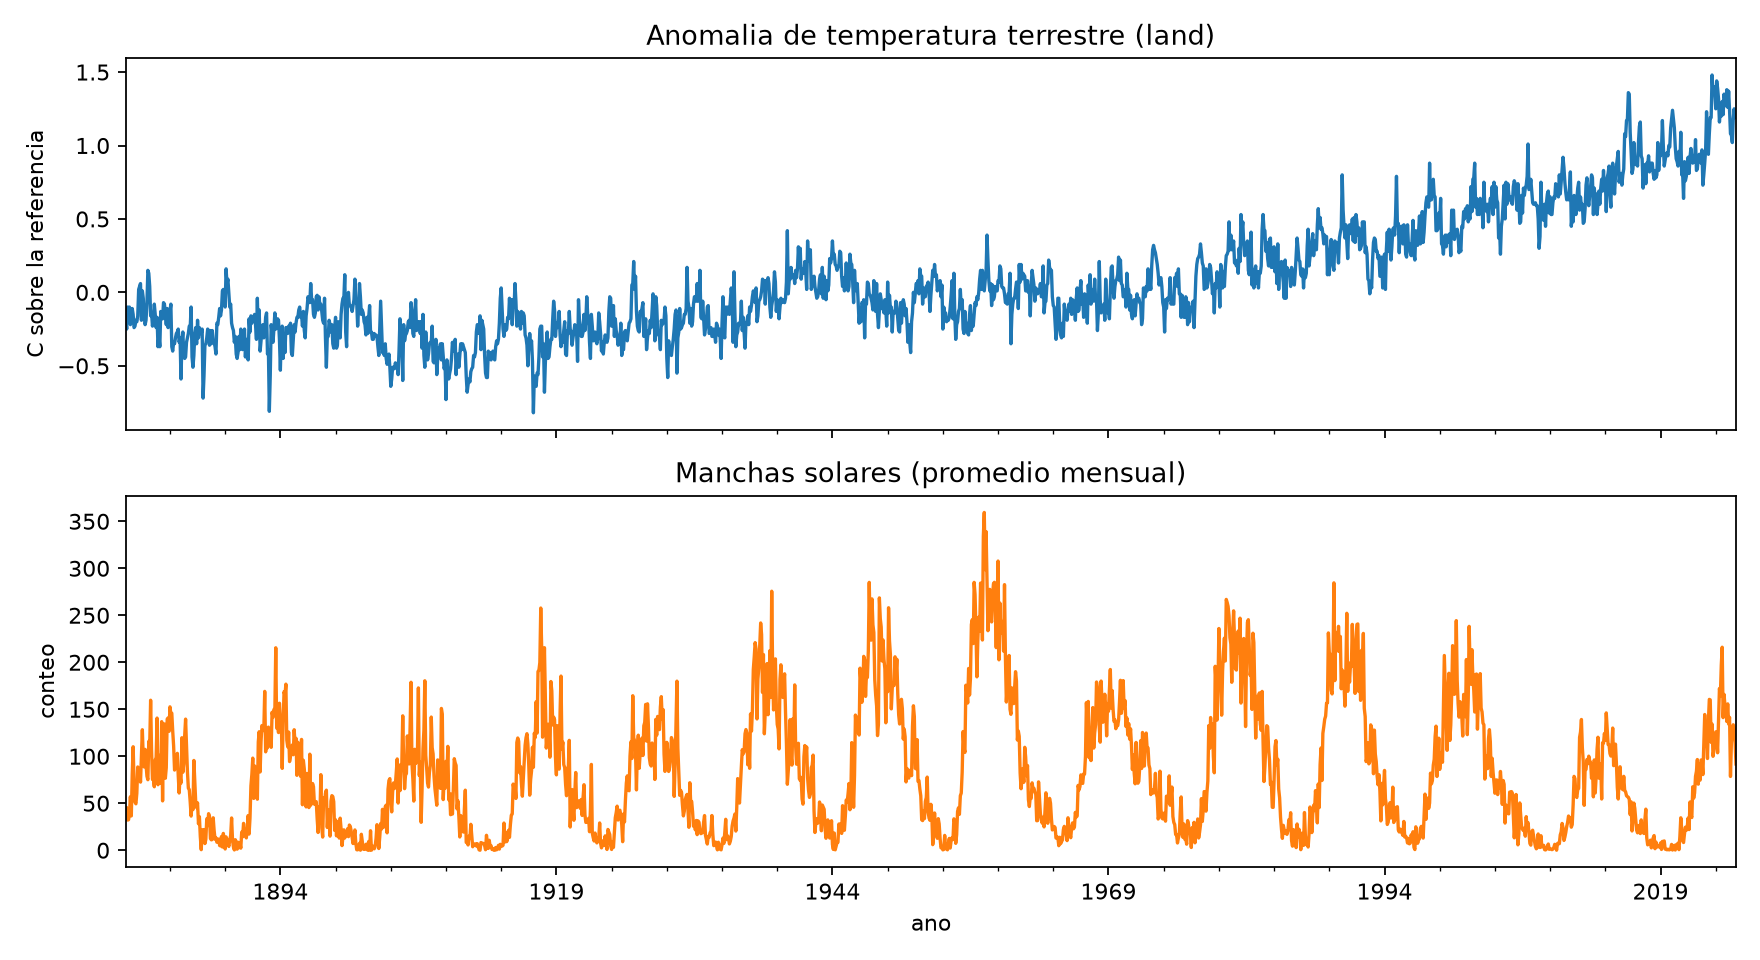
\includegraphics[width=0.85\linewidth]{assets/images/fig_nivel.png}
    \caption{Anomal\'ia terrestre \texttt{land} (arriba) y manchas solares mensuales (abajo), 1880--2025.}
    \label{fig:nivel}
  \end{figure*}

  La descomposici\'on aditiva de \texttt{land} con per\'iodo 12 (Figura~\ref{fig:descomposicion}) muestra una tendencia que recorre m\'as de un grado y un componente anual m\'inimo ($\pm 0.03\,^{\circ}\mathrm{C}$). Esa cifra hay que leerla con cuidado: \texttt{land} es un promedio global de tierra, y al descontar cada mes contra su climatolog\'ia el ciclo estacional ya est\'a parcialmente compensado entre hemisferios. Lo que sobrevive no es una estaci\'on meteorol\'ogica sino el residuo de esa compensaci\'on, que depende de cu\'anta tierra hay en cada hemisferio y no de un mecanismo clim\'atico; por eso la lectura (marzo $+0.025\,^{\circ}\mathrm{C}$, octubre $+0.023\,^{\circ}\mathrm{C}$, junio $-0.028\,^{\circ}\mathrm{C}$, con mediana en los mismos tres meses) no encaja con el verano del hemisferio norte y no debe interpretarse como se\~nal clim\'atica. La dispersi\'on por d\'ecada, en cambio, s\'i crece en las d\'ecadas recientes, y solo se ve midi\'endola sobre el residuo al que se le quitan la tendencia y el componente estacional, no sobre la serie cruda donde la pendiente la disfraza.

  \begin{figure*}[t]
    \centering
    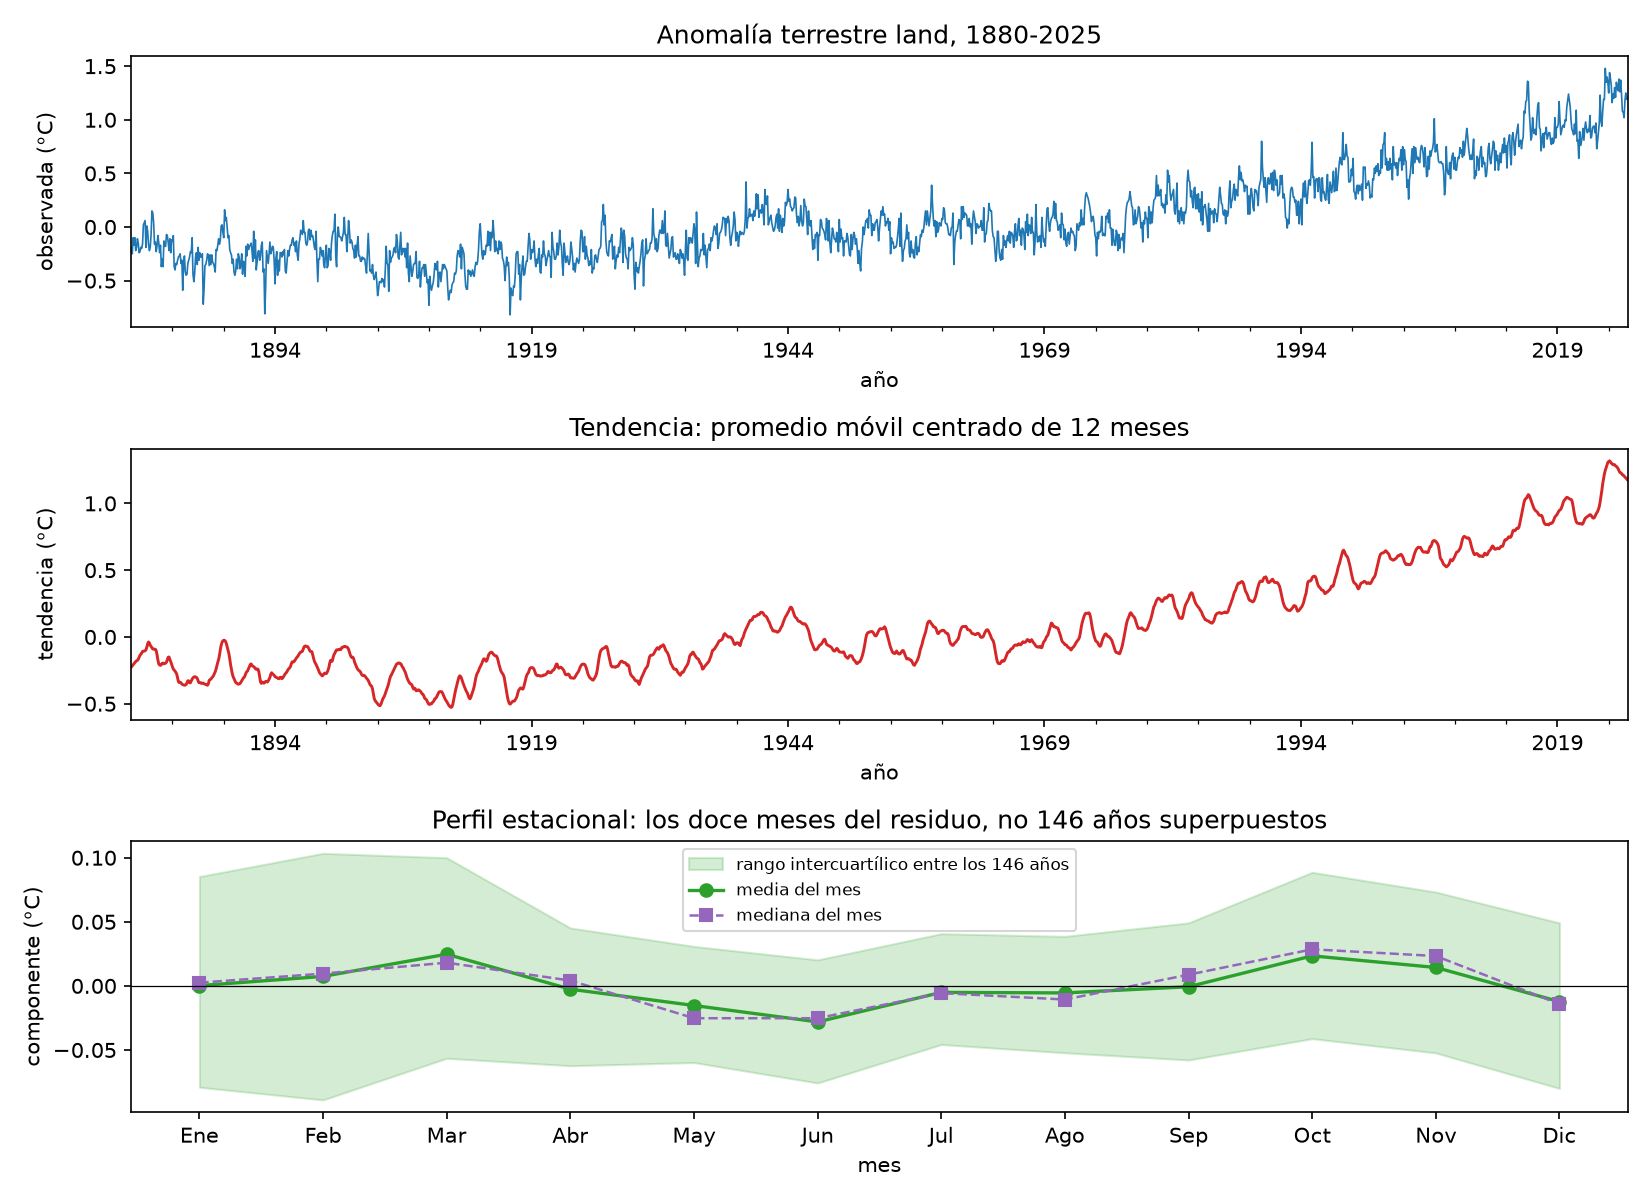
\includegraphics[width=0.85\linewidth]{assets/images/fig_descomposicion.png}
    \caption{Descomposici\'on aditiva de \texttt{land} con per\'iodo 12. Arriba, la serie observada; en el centro, la tendencia por promedio m\'ovil centrado de 12 meses; abajo, el perfil estacional del residuo, que son los doce meses del per\'iodo y no los 146 a\~nos superpuestos. La banda sombreada es el rango intercuart\'ilico de cada mes a lo largo del per\'iodo: es tres veces m\'as ancho que la l\'inea de media, que es la forma de ver que la estacionalidad es mucho menor que la variaci\'on entre a\~nos.}
    \label{fig:descomposicion}
  \end{figure*}

  El ciclo solar de unos once a\~nos es un rasgo mostrado de la serie \cite{hathaway2015} y se caracteriza pico a pico sobre la suavizada de 13 meses que usa el SILSO, exigiendo casi una d\'ecada entre m\'aximos porque cada ciclo trae picos dobles: 14 m\'aximos con un intervalo medio cercano a los 130 meses. Ese intervalo es una medida de distancia entre picos, no un an\'alisis espectral: el cuaderno no calcula periodograma ni densidad espectral, as\'i que la correspondencia con los 11 a\~nos can\'onicos viene del conteo de m\'aximos y no de una transformada. La Figura~\ref{fig:maximos} los marca.

  \begin{figure*}[t]
    \centering
    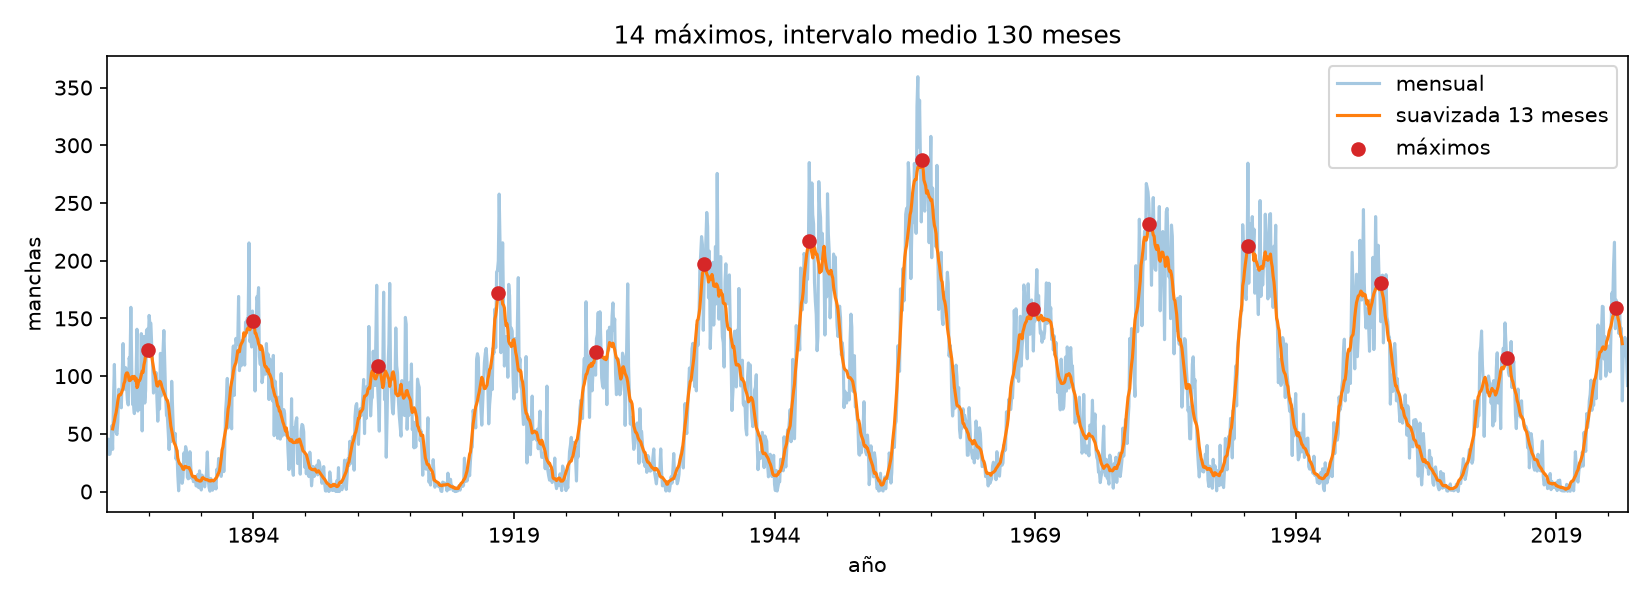
\includegraphics[width=0.85\linewidth]{assets/images/fig_maximos_solares.png}
    \caption{Manchas solares con los 14 m\'aximos del ciclo sobre la serie suavizada.}
    \label{fig:maximos}
  \end{figure*}

  El corte es estrictamente temporal: entreno 1880--2000 ($n=1\,452$) y prueba 2001 en adelante ($n=299$), sin barajar. La validaci\'on de la LSTM sale de dentro del entreno (1991--2000), sin tocar la prueba.

  \section{Metodolog\'ia}

  \subsection{ARIMA y ARIMAX}

  El test ADF \cite{dickey1979} sobre el entreno no rechaza ra\'iz unitaria en nivel ($p=0.42$) y s\'i en primera diferencia ($p\approx 0$), de modo que $d=1$. La ACF de la diferencia corta en el rezago uno y la PACF decae gradualmente, firma de media m\'ovil de orden uno; el AIC sobre el entreno elige ARIMA(2,1,1) frente a sus vecinos. El modelo pronostica como
  \begin{equation}
    \Delta y_t = \phi_1 \Delta y_{t-1} + \phi_2 \Delta y_{t-2} + \theta_1 \varepsilon_{t-1} + \varepsilon_t,
    \label{eq:arima}
  \end{equation}
  sin t\'ermino constante: con $d=1$ la diferenciaci\'on ya se lleva el nivel, y el modelo ajustado por el AIC no incluye ninguno. El ARIMAX a\~nade la mancha como regresor ex\'ogeno con el mismo orden y el mismo corte, de modo que P2 compara con sol contra sin sol; como $d=1$, la relaci\'on se estima sobre la serie diferenciada, y lo que se pone a prueba es si el aumento de la mancha en un mes acompa\~na el aumento de la anomal\'ia en ese mismo mes. Lo que aporta el sol es medible y es nulo: $\beta=-6.07\times10^{-6}$ con $p=0.96$ sobre el entreno, y el error en la prueba sube. P2 es una confirmaci\'on de lo que la correlaci\'on contempor\'anea del {EDA} ya hab\'ia anunciado, no un hallazgo que la pondere contradiga.

  \subsection{LSTM Univariada y Multivariada}

  La celda LSTM \cite{hochreiter1997} decide qu\'e olvidar, qu\'e guardar y qu\'e mostrar mediante sus compuertas:
  \begin{equation}
    C_t = f_t \odot C_{t-1} + i_t \odot \tilde{C}_t,
    \label{eq:lstm}
  \end{equation}
  donde $f_t$ e $i_t$ son las compuertas de olvido y entrada. La red (LSTM de 32 unidades m\'as capa densa) ve ventanas de 24 meses y pronostica la prueba de forma recursiva sin mirar sus datos; la versi\'on multivariada recibe adem\'as las manchas futuras observadas, como ex\'ogena que es \cite{lim2021}. Misma arquitectura, misma semilla, mismas ventanas: P3 es el \emph{ablation} que P2 dej\'o pendiente, y se repite con tres semillas porque el n\'umero exacto baila entre corridas aun con igual semilla (no-determinismo de GPU).

  \subsection{DQN sobre el P\'endulo}

  En \texttt{Pendulum-v1} \cite{gymnasium_pendulum}, sobre la interfaz est\'andar de \textsc{gymnasium} \cite{gymnasium2024}, el torque continuo se discretiza en cinco empujones y la red Q minimiza
  \begin{equation}
    L = \mathbb{E}\left[\left(r + \gamma \max_{a'} Q(s',a';\theta^{-}) - Q(s,a;\theta)\right)^2\right],
    \label{eq:dqn}
  \end{equation}
  con caja de recuerdos, red objetivo congelada y $\varepsilon$ decreciente durante 300 episodios. El list\'on es el agente al azar ($-1\,170\pm238$ de retorno medio en 20 episodios, con el entorno sembrado).

  \section{Resultados y Discusi\'on}

  La Tabla~\ref{tab:errores} resume la prueba y la Figura~\ref{fig:pronosticos} la dibuja. Antes de leerla hay que decirlo: la fila que gana no es un modelo, es copiar el mes anterior. La persistencia saca $0.1216$, y el ARIMA que sin ellas parecer\'ia el mejor se queda en $0.4637$, casi cuatro veces peor. La temperatura mensual es una serie suave y el error de un paso del ARIMA se realimenta a lo largo de 299 pasos de prueba. El drift lineal, que solo arrastra la pendiente histórica sin realimentar nada, tampoco ayuda: se queda en $0.5168$, incluso por detrás del ARIMA, porque extender el calentamiento en línea recta lo desvía un poco más cada año. As\'i que el margen de este trabajo no es predecir la temperatura, y el informe no lo reclama.

  Dentro de esa tabla, lo que si se sostiene es la pregunta del trabajo. P1: el ARIMA se predice con el propio pasado pero su pron\'ostico de horizonte largo se queda plano y no acompa\~na la subida. P2: el sol no aporta se\~nal, con $\beta=-6.07\times10^{-6}$, error est\'andar $1.13\times10^{-4}$ y $p=0.96$ sobre el entreno, y error mayor en la prueba ($\mathrm{RMSE}=0.5121$). P3: la LSTM sin sol empata al ARIMA y con sol pierde en las tres semillas. Que la red con m\'as informaci\'on pierda es el hallazgo que rompe la intuici\'on del trabajo, aunque parte de ese derrumbe sea la inestabilidad del rollout recursivo a ese horizonte y no el canal solar en s\'i.

  Todos los modelos quedan por debajo de una regla sin par\'ametros, y aun as\'i el sol nunca ayuda: por donde se mire, a\~adir las manchas cuesta error. Esa es la conclusi\'on del trabajo, y es un resultado negativo bien circunscrito, no una hip\'otesis sin probar.

  \begin{table}[t]
    \centering
    \caption{Error sobre la prueba 2001 en adelante ($n=299$). Las dos primeras filas no son modelos: son las reglas sin par\'ametros a las que todo lo demas deber\'ia ganarle.}
    \label{tab:errores}
    \begin{tabular}{lcc}
      \toprule
      Modelo & RMSE & MAE \\
      \midrule
      Persistencia $\hat y_{t}=y_{t-1}$ & \textbf{0.1216} & \textbf{0.0974} \\
      Drift lineal & 0.5168 & 0.4687 \\
      ARIMA(2,1,1) & 0.4637 & 0.3998 \\
      ARIMAX(2,1,1) con sol & 0.5121 & 0.4537 \\
      LSTM sin sol & 0.4799 & 0.4181 \\
      LSTM con sol & 0.9709 & 0.8770 \\
      \bottomrule
    \end{tabular}
  \end{table}

  \begin{figure*}[t]
    \centering
    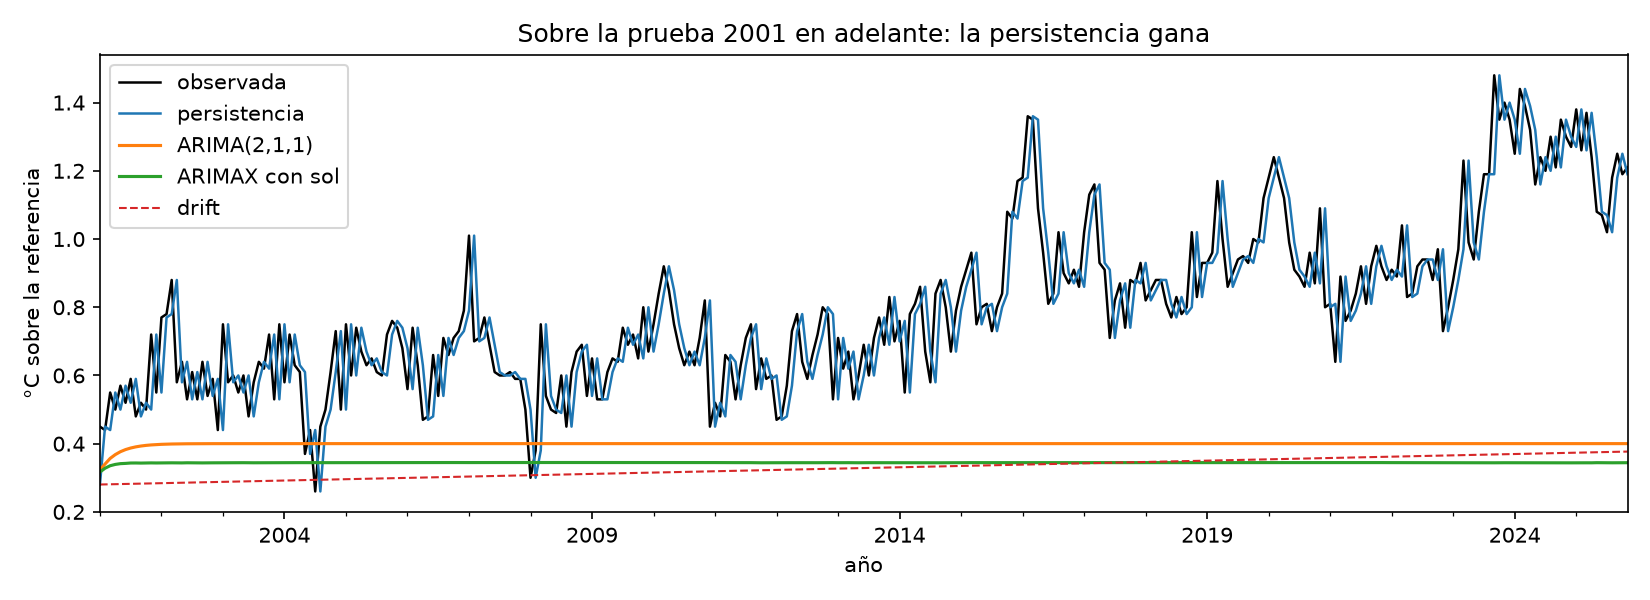
\includegraphics[width=0.85\linewidth]{assets/images/fig_pronosticos.png}
    \caption{Observada contra los cuatro pron\'osticos sobre la prueba: persistencia, drift, ARIMA y ARIMAX con sol. La l\'inea que se ajusta a la observada es la de persistencia.}
    \label{fig:pronosticos}
  \end{figure*}

  El bloque RL s\'i aprende: de nivel azar a retorno voraz $-183\pm108$ en la semilla principal y $-243\pm306$ y $-174\pm108$ en las dos de robustez, con la curva de la Figura~\ref{fig:curva}. La evaluaci\'on empareja los \'angulos iniciales del agente con los del azar, de modo que la comparaci\'on no es solo estad\'istica.

  \begin{figure}[t]
    \centering
    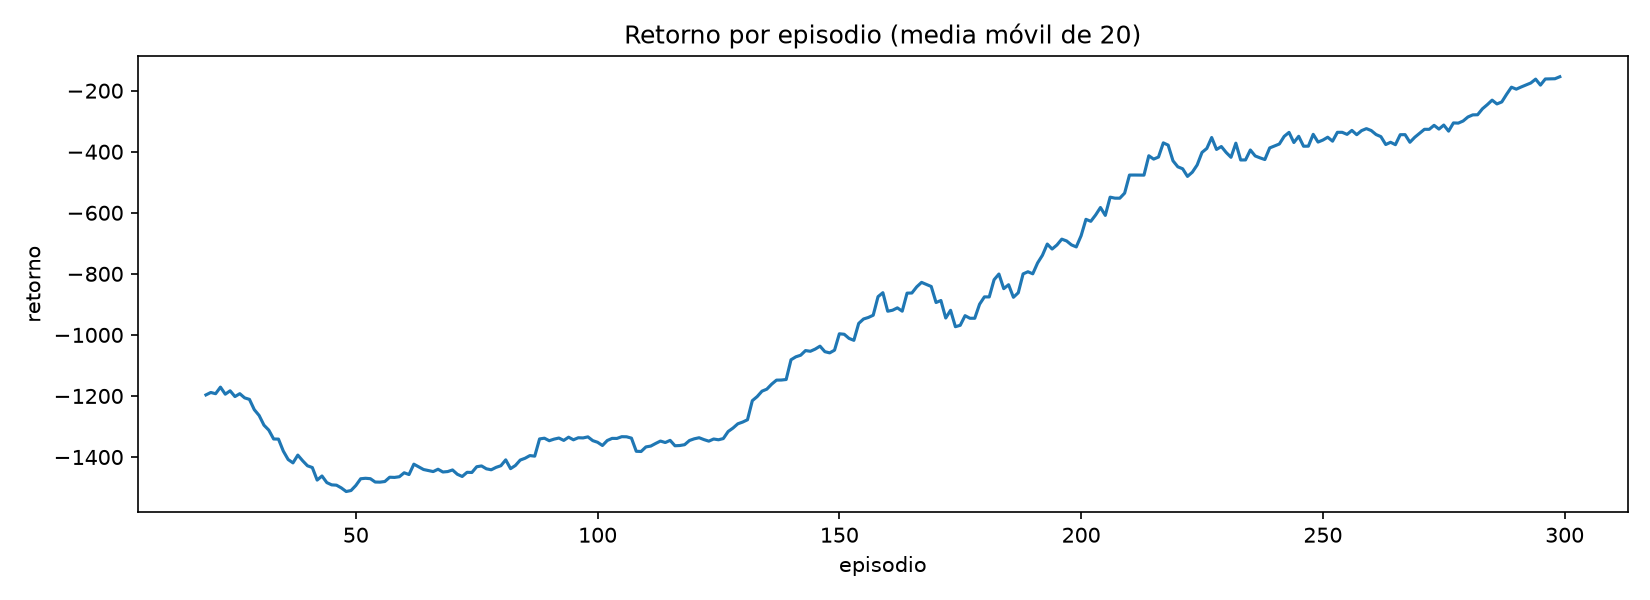
\includegraphics[width=\linewidth]{assets/images/fig_curva_rl.png}
    \caption{Retorno por episodio del DQN, media m\'ovil de 20.}
    \label{fig:curva}
  \end{figure}

  \section{Conclusiones}

  \begin{enumerate}
    \item La temperatura mensual no necesita un modelo: copiar el mes anterior la pronostica a $0.1216$ de RMSE, casi cuatro veces mejor que el ARIMA ajustado por AIC. Ninguno de los tres modelos aprendidos queda por encima de esa regla sin par\'ametros a 25 a\~nos de horizonte, y la otra regla sin par\'ametros, el drift lineal, tampoco la alcanza ($0.5168$, peor que el propio ARIMA), as\'i que este trabajo no demuestra que la serie sea dif\'acil de anticipar: demuestra que su historia lineal no es el problema.
    \item La actividad solar, con su ciclo decenal bien medido, no aporta se\~nal predictiva mensual a la temperatura en este marco. El {EDA} ya lo hab\'ia adelantado con la correlaci\'on contempor\'anea nula; P2 y P3 lo confirman en el modelo, con $\beta=-6.07\times10^{-6}$ y $p=0.96$ y con la red multivariada peor. Es una confirmaci\'on declarada, no un hallazgo nuevo.
    \item El aprendizaje por refuerzo s\'i resuelve su tarea continua cuando la recompensa gu\'ia paso a paso: el agente voraz llega a $-200\pm38$ de retorno medio entre las tres semillas frente a $-1170\pm238$ del azar, y la dispersi\'on entre semillas es menor que la dispersi\'on dentro de cada una, as\'i que la mejora es consistente y no un tirador afortunado. Lo que no se puede afirmar con tres semillas y cinco acciones discretas es que \'esto ocurra \emph{desde cualquier semilla}.
    \item Reproducibilidad: cuaderno ejecutado de punta a punta, con \texttt{requirements.txt} pinneado en local, las tres semillas fijadas en el entorno de \textsc{gymnasium} adem\'as de en \texttt{torch} y \texttt{numpy}, y las figuras exportadas por \texttt{export\_figures.py} a \texttt{assets/images/}. En Colab el cuaderno corre sin pines para no romper la imagen preinstalada, as\'i que ah\'i las cifras pueden variar en el orden del cuarto d\'ecimal; los valores citados salen de la corrida con \texttt{requirements.txt}. El cuaderno completo se ejecuta en Colab desde \enlacenb.
  \end{enumerate}

  \appendix
  Fragmentos de C\'odigo Clave

  Cada fragmento es el pasaje del cuaderno que sostiene una afirmaci\'on concreta del texto. Se reproducen tal cual, sin reescribir, para que las conclusiones se puedan verificar sin ejecutar el cuaderno.

  \textbf{A. La fecha decimal se trunca, no se redondea.}
  La columna \texttt{time} de Berkeley Earth viene como a\~no decimal. Redondearla salta febrero por completo, duplica abril y deja 585 fechas repetidas; el c\'alculo entero de a\~no y mes es lo que deja el marco en $1\,751$ meses \emph{unicos}, que es la base sobre la que est\'an calculadas la Tabla~\ref{tab:errores} y la Figura~\ref{fig:pronosticos}.

\begin{lstlisting}
tmp_year = tmp['time'].astype(int)
tmp_month = ((tmp['time'] - tmp_year) * 12).astype(int) + 1
tmp_month = tmp_month.clip(1, 12)
tmp['date'] = pd.to_datetime(dict(year=tmp_year, month=tmp_month, day=1))
tmp = tmp.set_index('date').sort_index()
  \end{lstlisting}

  \textbf{B. El escalador se ajusta sin ver la prueba.}
  El {\tt StandardScaler} se ajusta solo hasta 1990-12, dentro del bloque de ajuste; la transformaci\'on despu\'es se aplica a toda la serie, pero la media y la desviaci\'on vienen del pasado. Por eso el bloque de ventanas de la LSTM no filtra informaci\'on de 2001 en adelante.

\begin{lstlisting}
fit_end = '1990-12-01'
fit_frame = frame.loc[:fit_end]
scalers = {col: StandardScaler().fit(fit_frame[[col]])
           for col in ['land', 'sunspots']}
fit_mask = dates <= fit_end
val_mask = (dates > fit_end) & (dates <= '2000-12-01')
  \end{lstlisting}

  \textbf{C. El pron\'ostico es recursivo y arranca en el borde del entreno.}
  No hay teacher forcing: cada paso del 2001 al 2025 se alimenta de la predicci\'on anterior, no del valor observado. Los 299 pasos de realimentaci\'on son la raz\'on de que la LSTM multivariada termine colapsando y la raz\'on tambi\'en de que el ARIMA pierda frente a la persistencia: el error de un paso se acumula durante todo el horizonte.

\begin{lstlisting}
history = list(data[len(fit_frame) - window:len(train)])
upcoming_sun = scaled.loc[test.index, 'sunspots'].values
with torch.no_grad():
    for step in range(len(test)):
        features = torch.Tensor(np.array(history[-window:])[None]).to(device)
        guess = float(net(features))
        if len(columns) == 1:
            history.append([guess])
        else:
            history.append([guess, upcoming_sun[step]])
  \end{lstlisting}

  \textbf{D. Las dos l\'ineas base.}
  Es el fragmento que decide el marco del trabajo: sin estas dos reglas, la comparaci\'on de la Tabla~\ref{tab:errores} se hace entre modelos y no dice nada sobre si alguno de ellos es mejor que no hacer nada.

\begin{lstlisting}
persistence = frame['land'].shift(1).loc[test.index]
slope = (train['land'].iloc[-1] - train['land'].iloc[0]) / (len(train) - 1)
drift = pd.Series(train['land'].iloc[-1] + slope * np.arange(1, len(test) + 1),
                  index=test.index)
  \end{lstlisting}

  \textbf{E. La evidencia del resultado central.}
  El p-valor del coeficiente solar se calcula sobre el bloque de ajuste y se imprime antes de mirar la m\'etrica de la prueba, que es el orden honesto: si se mira el RMSE primero, la interpretaci\'on ya viene sesgada.

\begin{lstlisting}
coef = exog_fit.params['sunspots']
err = exog_fit.bse['sunspots']
pval = exog_fit.pvalues['sunspots']
  \end{lstlisting}

  \textbf{F. El entorno de \textsc{gymnasium} tambi\'en va sembrado.}
  \texttt{torch.manual\_seed} y \texttt{numpy.seed} no controlan el estado inicial de un entorno: \texttt{gym.make} no acepta \texttt{seed}, que hay que pasar a \texttt{reset}. Sin esto, el agente al azar y el agente voraz no comparten los \'angulos de partida y la comparaci\'on de la Figura~\ref{fig:curva} no es pareada.

\begin{lstlisting}
eval_env = gym.make('Pendulum-v1')
for episode in range(20):
    observation, _ = eval_env.reset(seed=EVAL_SEED + episode)
  \end{lstlisting}

  \textbf{G. Exportaci\'on de las figuras.}
  Las cinco figuras del informe salen de este script, no del cuaderno: el cuaderno calcula y muestra, el script escribe en \texttt{assets/images/}.

\begin{lstlisting}
./venv/bin/python export_figures.py
  \end{lstlisting}

  \bibliographystyle{IEEEtran}
  \bibliography{bib/references}

\end{document}
